\section{独立非同分布情形}
\label{sec:clt-non-identical}

一批测量由精度不同的仪器完成，各次误差独立，方差却各不相同；或者每一项的分布本身随总项数变化，像第~\ref{sec:clt-standardization}节的特制硬币。这时没有共同的$\sigma$，标准化只能用总和的标准差。问题变成：各项方差不同，甚至分布随规模改变，什么时候和仍然近似高斯？上一节的特制硬币说明答案不会是“总是”，需要一个条件把“少数几项决定总和”的情形排除掉。

\subsection{三角阵与总方差}
\label{sec:clt-triangular}

各项的分布可以随规模$n$改变，所以把每个规模下的求和项单独列成一行。

\begin{definition}[三角阵]
\label{def:clt-triangular-array}
对每个$n\geq1$，设$k_n$是正整数，$X_{n,1},\dots,X_{n,k_n}$是一组相互独立的随机变量，满足
\begin{equation}
 \mathbb{E}[X_{n,k}]=0,\qquad \sigma_{n,k}^2=\operatorname{Var}(X_{n,k})<\infty .
 \label{eq:clt-array-moments}
\end{equation}
记第$n$行的和与总方差为
\begin{equation}
 S_n=\sum_{k=1}^{k_n}X_{n,k},\qquad s_n^2=\sum_{k=1}^{k_n}\sigma_{n,k}^2 ,
 \label{eq:clt-row-variance}
\end{equation}
并要求$0<s_n^2<\infty$。这样的一族随机变量称为\term{三角阵}（triangular array）。
\end{definition}

名字来自$k_n=n$时的排列方式：第$n$行有$n$项，各行左对齐排成三角形，见图~\ref{fig:clt-triangular-array}。定义只要求同一行内的变量相互独立，不要求不同行之间独立，甚至不要求它们定义在同一个概率空间上。原因是我们只关心每一行的和$S_n$的分布，而$S_n$的分布只由第$n$行的联合分布决定。

\begin{BookInlineFigure}
 \centering
 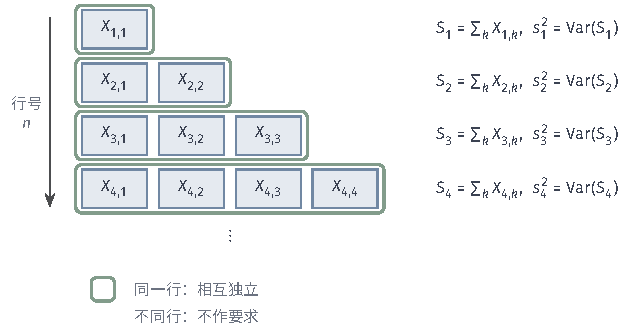
\includegraphics[width=107mm]{figures/07-probability/03-probability-limits/tikz/clt-triangular-array/figure.pdf}
 \caption{三角阵的结构（图中取$k_n=n$）。每一行是一组中心化的求和项，绿框表示行内相互独立；行和$S_n$与总方差$s_n^2$逐行计算，不同行之间不作任何要求。}
 \label{fig:clt-triangular-array}
\end{BookInlineFigure}

由行内独立，$\operatorname{Var}(S_n)=s_n^2$。把各项除以$s_n$，
\[
 \sum_{k=1}^{k_n}\operatorname{Var}\Bigl(\frac{X_{n,k}}{s_n}\Bigr)=\frac{1}{s_n^2}\sum_{k=1}^{k_n}\sigma_{n,k}^2=1 ,
\]
归一化后的各项方差之和为一，$S_n/s_n$均值为零、方差为一。比值$\sigma_{n,k}^2/s_n^2$就是第$k$项在总方差中所占的份额。

\paragraph{独立同分布是特例}
定理~\ref{thm:clt-iid}的情形可以写成三角阵：取$k_n=n$，$X_{n,k}=X_k-\mu$，与$n$无关，则$s_n^2=n\sigma^2$，$S_n/s_n=Z_n$。每一行只是上一行再加一项。三角阵的一般性在于允许各项随$n$整体改变。

\paragraph{三个例子}
本节用下面三个三角阵检验各个条件，它们都满足定义~\ref{def:clt-triangular-array}。
\begin{itemize}
 \item 例A：$X_{n,k}\sim\operatorname{Unif}(-k,k)$，$k=1,\dots,n$。各项有界，方差为$k^2/3$，越往后越大。由$\sum_{k=1}^{n}k^2=n(n+1)(2n+1)/6$，
 \[
  s_n^2=\frac{n(n+1)(2n+1)}{18} .
 \]
 \item 例B：$X_{n,k}\sim\mathcal{N}(0,2^{k})$，$k=1,\dots,n$。方差逐项加倍，$s_n^2=2^{n+1}-2$，最后一项约占总方差的一半。
 \item 例C：$X_{n,k}=B_{n,k}-1/n$，$B_{n,k}\sim\operatorname{Bern}(1/n)$，$k=1,\dots,n$。这是特制硬币的中心化，各项方差都是$\frac1n(1-\frac1n)$，$s_n^2=1-1/n$。
\end{itemize}
例C的行和是$S_n=\operatorname{Bin}(n,1/n)-1$，第~\ref{sec:clt-standardization}节已经看到它的极限不是高斯分布。例B的各项是独立高斯变量，由第~\ref{chap:multivariate-distributions}章，它们的和仍是高斯变量，$S_n\sim\mathcal{N}(0,s_n^2)$，于是对每个$n$都有$S_n/s_n\sim\mathcal{N}(0,1)$。

\subsection{Lindeberg条件}
\label{sec:clt-lindeberg}

例C的毛病在于：总和的波动几乎全部来自“偶尔取到大值”的项。每一项$X_{n,k}$以概率$1/n$取值$1-1/n$，这个值与行的标准差$s_n\approx1$同阶。把方差按取值的大小拆开，例C的方差几乎全部来自那些与$s_n$同阶的取值。要排除这种情形，就要求方差中来自“大值”的部分可以忽略。

\paragraph{截断二阶矩}
固定$\varepsilon>0$，把“大值”理解为绝对值超过$\varepsilon s_n$的取值。每一项的方差拆成两部分，
\[
 \sigma_{n,k}^2=\mathbb{E}\bigl[X_{n,k}^2\mathbf{1}_{\{\lvert X_{n,k}\rvert\leq\varepsilon s_n\}}\bigr]+\mathbb{E}\bigl[X_{n,k}^2\mathbf{1}_{\{\lvert X_{n,k}\rvert>\varepsilon s_n\}}\bigr] .
\]
后一部分是大值贡献的方差。把整行的这部分加起来，再除以总方差，得到大值贡献的份额
\begin{equation}
 L_n(\varepsilon)=\frac{1}{s_n^2}\sum_{k=1}^{k_n}\mathbb{E}\bigl[X_{n,k}^2\mathbf{1}_{\{\lvert X_{n,k}\rvert>\varepsilon s_n\}}\bigr] .
 \label{eq:clt-lindeberg-ratio}
\end{equation}
$L_n(\varepsilon)$在$0$和$1$之间，随$\varepsilon$增大而不增。

\begin{definition}[Lindeberg条件]
\label{def:clt-lindeberg}
称三角阵满足\term{Lindeberg条件}（Lindeberg condition），如果对每个$\varepsilon>0$，
\begin{equation}
 L_n(\varepsilon)\to0\qquad(n\to\infty) .
 \label{eq:clt-lindeberg}
\end{equation}
\end{definition}

条件要求对每个$\varepsilon$都成立，$\varepsilon$越小，被算作大值的范围越宽，要求越严。它说的是：无论把门槛定在总标准差的多小一个比例上，越过门槛的取值所贡献的方差都终将可以忽略。

\paragraph{它推出单项份额趋零}
Lindeberg条件首先保证没有哪一项的方差占总方差的可观份额。对每一项，把方差按$\lvert X_{n,k}\rvert\leq\varepsilon s_n$与否拆开：前一部分不超过$\varepsilon^2s_n^2$，后一部分不超过整行大值贡献之和$s_n^2L_n(\varepsilon)$。于是
\begin{equation}
 \max_{1\leq k\leq k_n}\frac{\sigma_{n,k}^2}{s_n^2}\leq\varepsilon^2+L_n(\varepsilon) .
 \label{eq:clt-max-share}
\end{equation}
令$n\to\infty$，右边的上极限不超过$\varepsilon^2$；$\varepsilon$任意，所以最大份额趋于零。反过来不成立：例C的每一项份额都是$1/n$，趋于零，Lindeberg条件却不成立。单项方差小，不等于大值的贡献小。

\begin{theorem}[Lindeberg中心极限定理]
\label{thm:clt-lindeberg}
设三角阵满足Lindeberg条件~\eqref{eq:clt-lindeberg}。则
\begin{equation}
 \frac{S_n}{s_n}\xrightarrow{\mathrm{d}}\mathcal{N}(0,1) .
 \label{eq:clt-lindeberg-limit}
\end{equation}
\end{theorem}

证明的结构与定理~\ref{thm:clt-iid}相同，仍是比较特征函数的乘积。不同之处在于各因子不再相同，余项要逐项估计后再求和；Lindeberg条件正好控制余项之和。

\begin{proof}
把$X_{n,k}$换成$X_{n,k}/s_n$，可以设$s_n=1$，这时式~\eqref{eq:clt-lindeberg-ratio}中的门槛就是$\varepsilon$。固定$t$和$\varepsilon\in(0,1)$，记$\phi_{n,k}$为$X_{n,k}$的特征函数，并令
\[
 w_{n,k}=1-\frac{t^2\sigma_{n,k}^2}{2} .
\]

第一步，单项误差。在式~\eqref{eq:clt-exp-remainder}中令$x=tX_{n,k}$取期望，与定理~\ref{thm:clt-iid}证明的第一步相同，得到
\[
 \lvert\phi_{n,k}(t)-w_{n,k}\rvert\leq\mathbb{E}\Bigl[\min\Bigl\{\frac{\lvert t\rvert^{3}\lvert X_{n,k}\rvert^{3}}{6},\ t^2X_{n,k}^2\Bigr\}\Bigr] .
\]
在$\{\lvert X_{n,k}\rvert\leq\varepsilon\}$上用三次界，并利用$\lvert X_{n,k}\rvert^3\leq\varepsilon X_{n,k}^2$；在其余部分用二次界。于是
\[
 \lvert\phi_{n,k}(t)-w_{n,k}\rvert\leq\frac{\lvert t\rvert^{3}\varepsilon}{6}\sigma_{n,k}^2+t^2\,\mathbb{E}\bigl[X_{n,k}^2\mathbf{1}_{\{\lvert X_{n,k}\rvert>\varepsilon\}}\bigr] .
\]

第二步，求和。对$k$求和，由$\sum_k\sigma_{n,k}^2=1$与式~\eqref{eq:clt-lindeberg-ratio}，
\[
 \sum_{k=1}^{k_n}\lvert\phi_{n,k}(t)-w_{n,k}\rvert\leq\frac{\lvert t\rvert^{3}\varepsilon}{6}+t^2L_n(\varepsilon) .
\]

第三步，比较乘积。由式~\eqref{eq:clt-max-share}，最大份额趋于零，所以$n$充分大时每个$t^2\sigma_{n,k}^2\leq2$，从而$\lvert w_{n,k}\rvert\leq1$。由行内独立，$\phi_{S_n}(t)=\prod_k\phi_{n,k}(t)$。用引理~\ref{lem:clt-product-difference}，
\[
 \Bigl\lvert\phi_{S_n}(t)-\prod_{k=1}^{k_n}w_{n,k}\Bigr\rvert\leq\frac{\lvert t\rvert^{3}\varepsilon}{6}+t^2L_n(\varepsilon) .
\]
令$n\to\infty$，右边趋于$\lvert t\rvert^3\varepsilon/6$。$\varepsilon$可以任意小，所以左边趋于零。

第四步，乘积的极限。记$a_k=t^2\sigma_{n,k}^2/2\geq0$，则$\sum_ka_k=t^2/2$，而
\[
 \mathrm{e}^{-t^2/2}=\prod_{k=1}^{k_n}\mathrm{e}^{-a_k} .
\]
对$a\geq0$，由带余项的Taylor公式，$\mathrm{e}^{-a}=1-a+\mathrm{e}^{-\xi}a^2/2$，其中$\xi\in(0,a)$，所以$\lvert\mathrm{e}^{-a}-(1-a)\rvert\leq a^2/2$。$\mathrm{e}^{-a_k}$与$w_{n,k}=1-a_k$的模都不超过$1$，再用引理~\ref{lem:clt-product-difference}，
\[
 \Bigl\lvert\prod_{k}w_{n,k}-\mathrm{e}^{-t^2/2}\Bigr\rvert\leq\sum_k\frac{a_k^2}{2}\leq\frac{\max_ka_k}{2}\sum_ka_k=\frac{t^4}{8}\max_k\sigma_{n,k}^2 .
\]
最大份额趋于零，右边趋于零。

第三、四步合起来，$\phi_{S_n}(t)\to\mathrm{e}^{-t^2/2}$对每个$t$成立，由连续性定理得到式~\eqref{eq:clt-lindeberg-limit}。
\end{proof}

证明中Lindeberg条件出现在第三步：小值部分用三次界，贡献至多$\varepsilon$；大值部分只能用二次界，贡献正是$L_n(\varepsilon)$。第四步还需要每项份额都小，这由式~\eqref{eq:clt-max-share}从Lindeberg条件推出。

\paragraph{独立同分布的情形}
对定理~\ref{thm:clt-iid}的三角阵，$Y=(X_1-\mu)/\sigma$，各项同分布，
\[
 L_n(\varepsilon)=\frac{1}{n\sigma^2}\cdot n\,\mathbb{E}\bigl[(X_1-\mu)^2\mathbf{1}_{\{\lvert X_1-\mu\rvert>\varepsilon\sigma\sqrt{n}\}}\bigr]
 =\mathbb{E}\bigl[Y^2\mathbf{1}_{\{\lvert Y\rvert>\varepsilon\sqrt{n}\}}\bigr] .
\]
被积函数被$Y^2$控制，并对每个样本点最终为零，由支配收敛定理，$L_n(\varepsilon)\to0$。所以定理~\ref{thm:clt-iid}是定理~\ref{thm:clt-lindeberg}的特例，二阶矩有限恰好就是独立同分布时的Lindeberg条件。

\paragraph{三个例子的核验}
图~\ref{fig:clt-lindeberg-shares}取$n=20$，$\varepsilon=0.5$，把每一项的方差份额$\sigma_{n,k}^2/s_n^2$画成柱，柱中红色部分是大值的贡献，红色部分之和就是$L_{20}(0.5)$。三个例子的结果分别是
\[
 \text{A}:\ 0.208,\qquad \text{B}:\ 0.749,\qquad \text{C}:\ 0.95 .
\]

\begin{BookInlineFigure}
 \centering
 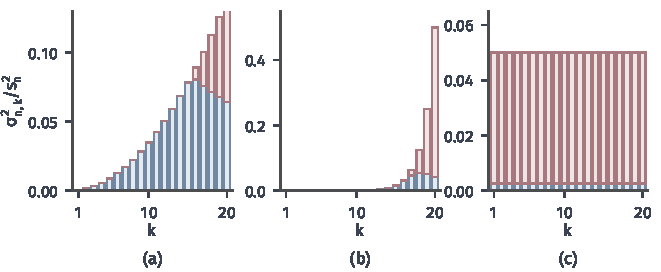
\includegraphics[width=112mm]{figures/07-probability/03-probability-limits/matplotlib/clt-lindeberg-shares/figure.pdf}
 \caption{$n=20$、$\varepsilon=0.5$时各项的方差份额$\sigma_{n,k}^2/s_n^2$。蓝色部分来自$\lvert X_{n,k}\rvert\leq\varepsilon s_n$的取值，红色部分来自$\lvert X_{n,k}\rvert>\varepsilon s_n$的取值，红色之和为$L_{20}(0.5)$。(a)例A，$\operatorname{Unif}(-k,k)$；(b)例B，$\mathcal{N}(0,2^{k})$；(c)例C，中心化的$\operatorname{Bern}(1/20)$。纵轴刻度各不相同。}
 \label{fig:clt-lindeberg-shares}
\end{BookInlineFigure}

例A中$s_{20}^2\approx956.7$，门槛$\varepsilon s_{20}\approx15.5$，只有$k\geq16$的几项可能越过门槛。$\operatorname{Unif}(-k,k)$越过$c<k$的部分贡献
\[
 \mathbb{E}\bigl[X^2\mathbf{1}_{\{\lvert X\rvert>c\}}\bigr]=2\int_c^k\frac{x^2}{2k}\,\mathrm{d}x=\frac{k^3-c^3}{3k} .
\]
代入$c=\varepsilon s_{20}\approx15.465$，$k=16,\dots,20$五项越过门槛的贡献依次约为
\[
 8.28,\quad 23.81,\quad 39.51,\quad 55.44,\quad 71.69 ,
\]
合计约$198.7$，除以$s_{20}^2\approx956.7$得$L_{20}(0.5)\approx0.208$。越往后的项方差越大，越过门槛的部分也越多，图中红色集中在右端。

随着$n$增大，门槛$\varepsilon s_n$按$n^{3/2}$增长，而各项的取值不超过$n$。对$\varepsilon=0.5$，从$n=35$起$\varepsilon s_n\geq n$，没有任何一项能越过门槛，$L_n(0.5)=0$。对任意固定的$\varepsilon>0$同样如此，所以例A满足Lindeberg条件，$S_n/s_n\xrightarrow{\mathrm{d}}\mathcal{N}(0,1)$。

例C中门槛$0.5s_n$小于$0.5$。$n\geq3$时，每一项以概率$1/n$取到的值$1-1/n$越过门槛，另一个取值$-1/n$不越过。所以
\[
 L_n(0.5)=\frac{1}{s_n^2}\cdot n\cdot\frac1n\Bigl(1-\frac1n\Bigr)^{2}=1-\frac1n\to1 .
\]
条件不成立，极限也确实不是高斯分布。

\paragraph{不是必要条件}
例B的$L_n(0.5)$稳定在$0.749$附近，Lindeberg条件不成立，可是$S_n/s_n$对每个$n$都恰好服从$\mathcal{N}(0,1)$。原因是例B的大项本身就是高斯的：最后一项独占一半方差，它的形状直接留在和里，而它碰巧是钟形。所以Lindeberg条件是充分条件，不是中心极限定理的必要条件。

图~\ref{fig:clt-lindeberg-ratio}画出三个例子的$L_n(0.5)$与最大份额随$n$的变化。例A两条曲线都趋于零；例B两条都不趋于零；例C的最大份额$1/n$趋于零，$L_n$却趋于一。

\begin{BookInlineFigure}
 \centering
 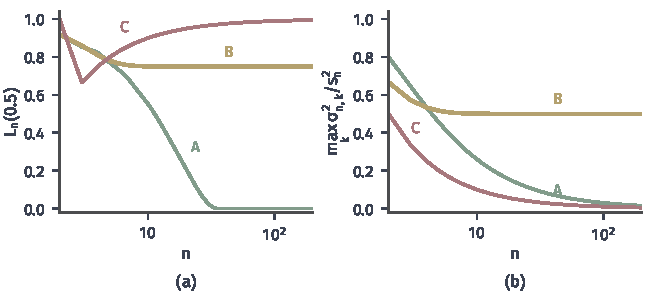
\includegraphics[width=112mm]{figures/07-probability/03-probability-limits/matplotlib/clt-lindeberg-ratio/figure.pdf}
 \caption{三个三角阵的(a)Lindeberg比值$L_n(0.5)$与(b)最大方差份额$\max_k\sigma_{n,k}^2/s_n^2$，$n=2,\dots,200$，横轴为对数刻度。绿为例A，黄为例B，红为例C。}
 \label{fig:clt-lindeberg-ratio}
\end{BookInlineFigure}

例B也说明了缺什么才能反推。若最大份额趋于零，并且$S_n/s_n\xrightarrow{\mathrm{d}}\mathcal{N}(0,1)$，则Lindeberg条件一定成立，这是Feller的逆定理，证明需要更细的特征函数估计，篇幅较长，读者可查阅~\scite{math-kallenberg2021probability}。在“没有一项占优”的前提下，Lindeberg条件就是高斯极限的充要条件；例B不满足这个前提，所以不构成矛盾。

\subsection{Lyapunov条件}
\label{sec:clt-lyapunov}

核验Lindeberg条件要计算截断二阶矩，像例A那样对每一项求越过门槛的部分，往往并不方便。如果各项有略高于二阶的矩，可以用一个更容易计算的量代替它。

\paragraph{用高阶矩压住截断}
在$\{\lvert x\rvert>\varepsilon s_n\}$上，$\lvert x\rvert/(\varepsilon s_n)>1$，于是对任意$\delta>0$，
\[
 x^2\leq x^2\Bigl(\frac{\lvert x\rvert}{\varepsilon s_n}\Bigr)^{\delta}=\frac{\lvert x\rvert^{2+\delta}}{\varepsilon^{\delta}s_n^{\delta}} .
\]
截断二阶矩因此不超过$2+\delta$阶绝对矩除以$\varepsilon^{\delta}s_n^{\delta}$。门槛越高，越过它的取值越大，高阶矩对它们的加权越重，这个不等式正是利用了这一点。

\begin{theorem}[Lyapunov中心极限定理]
\label{thm:clt-lyapunov}
设三角阵的各项具有有限的$2+\delta$阶绝对矩，其中$\delta>0$固定，并且
\begin{equation}
 \Lambda_n(\delta)=\frac{1}{s_n^{2+\delta}}\sum_{k=1}^{k_n}\mathbb{E}\bigl[\lvert X_{n,k}\rvert^{2+\delta}\bigr]\to0 .
 \label{eq:clt-lyapunov}
\end{equation}
则Lindeberg条件成立，从而$S_n/s_n\xrightarrow{\mathrm{d}}\mathcal{N}(0,1)$。
\end{theorem}

条件~\eqref{eq:clt-lyapunov}称为\term{Lyapunov条件}（Lyapunov condition）。

\begin{proof}
对每一项用上面的不等式再取期望，并对$k$求和，
\[
 L_n(\varepsilon)\leq\frac{1}{s_n^2}\sum_{k=1}^{k_n}\frac{\mathbb{E}\bigl[\lvert X_{n,k}\rvert^{2+\delta}\bigr]}{\varepsilon^{\delta}s_n^{\delta}}=\frac{\Lambda_n(\delta)}{\varepsilon^{\delta}} .
\]
对每个固定的$\varepsilon>0$，右边趋于零，这就是Lindeberg条件。再由定理~\ref{thm:clt-lindeberg}得到结论。
\end{proof}

\paragraph{例A的三阶矩}
取$\delta=1$。$\operatorname{Unif}(-k,k)$的三阶绝对矩是
\[
 \mathbb{E}\bigl[\lvert X\rvert^{3}\bigr]=\frac{1}{2k}\int_{-k}^{k}\lvert x\rvert^{3}\,\mathrm{d}x=\frac{k^3}{4} .
\]
由$\sum_{k=1}^{n}k^3=\bigl(n(n+1)/2\bigr)^2$与$s_n^2=n(n+1)(2n+1)/18$，
\[
 \Lambda_n(1)=\frac{n^2(n+1)^2/16}{\bigl(n(n+1)(2n+1)/18\bigr)^{3/2}}\approx\frac{27}{16\sqrt{n}} .
\]
$n=20,100,1000$时，精确值分别约为$0.373$、$0.168$、$0.053$，按$1/\sqrt{n}$趋于零。这里不需要像核验Lindeberg条件那样找出哪些项越过门槛，只要把各项的矩加起来。

\paragraph{有界项}
若存在常数$M$使$\lvert X_{n,k}\rvert\leq M$，并且$s_n\to\infty$，则$\lvert X_{n,k}\rvert^3\leq MX_{n,k}^2$，取期望得
\[
 \mathbb{E}\bigl[\lvert X_{n,k}\rvert^{3}\bigr]\leq M\sigma_{n,k}^2 .
\]
对$k$求和再除以$s_n^3$，
\[
 \Lambda_n(1)\leq\frac{M s_n^2}{s_n^3}=\frac{M}{s_n}\to0 .
\]
所以总方差趋于无穷的一致有界独立项，标准化和总趋于标准高斯分布。例C的各项也有界，但$s_n^2=1-1/n$不趋于无穷，这个推理不适用。

\paragraph{两个条件的比较}
Lyapunov条件多要求了$2+\delta$阶矩，换来的是只需计算未截断的矩之和。它比Lindeberg条件严格地强：设$X_1,X_2,\dots$独立同分布，方差有限，但对每个$\delta>0$都有$\mathbb{E}[\lvert X_1\rvert^{2+\delta}]=\infty$，例如密度在$\lvert x\rvert>\mathrm{e}$上与$1/(\lvert x\rvert^3\ln^2\lvert x\rvert)$成正比的对称分布。这时Lyapunov条件无从谈起，而独立同分布时Lindeberg条件总成立，中心极限定理照样成立。图~\ref{fig:clt-condition-map}汇总了本节的几个条件与结论之间的推出关系。

\begin{BookInlineFigure}
 \centering
 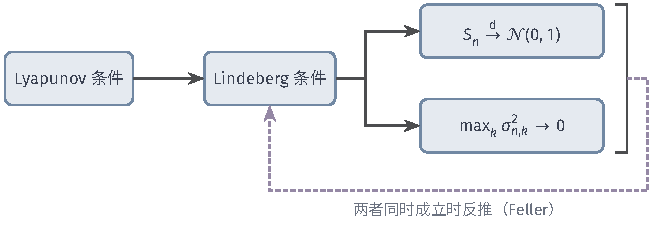
\includegraphics[width=111mm]{figures/07-probability/03-probability-limits/tikz/clt-condition-map/figure.pdf}
 \caption{三角阵各条件与结论的关系（行内独立、中心化、$s_n=1$）。实线箭头表示推出；紫色虚线表示Feller逆定理：高斯极限与最大份额趋零同时成立时，可以反推Lindeberg条件。单有高斯极限推不出Lindeberg条件，例B即是。}
 \label{fig:clt-condition-map}
\end{BookInlineFigure}

这些条件都只是充分条件，或者在附加前提下才是充要条件。把它们当作中心极限定理的必要条件，就会像例B那样误判；反过来，看到“每项方差都很小”就断言高斯极限，又会在例C上出错。
